\documentclass{ximera}

 

\usepackage{epsfig}

\graphicspath{
  {./}
  {figures/}
}

\usepackage{morewrites}
\makeatletter
\newcommand\subfile[1]{%
\renewcommand{\input}[1]{}%
\begingroup\skip@preamble\otherinput{#1}\endgroup\par\vspace{\topsep}
\let\input\otherinput}
\makeatother

\newcommand{\includeexercises}{\directlua{dofile("/home/jim/linearAlgebra/laode/exercises.lua")}}

%\newcounter{ccounter}
%\setcounter{ccounter}{1}
%\newcommand{\Chapter}[1]{\setcounter{chapter}{\arabic{ccounter}}\chapter{#1}\addtocounter{ccounter}{1}}

%\newcommand{\section}[1]{\section{#1}\setcounter{thm}{0}\setcounter{equation}{0}}

%\renewcommand{\theequation}{\arabic{chapter}.\arabic{section}.\arabic{equation}}
%\renewcommand{\thefigure}{\arabic{chapter}.\arabic{figure}}
%\renewcommand{\thetable}{\arabic{chapter}.\arabic{table}}

%\newcommand{\Sec}[2]{\section{#1}\markright{\arabic{ccounter}.\arabic{section}.#2}\setcounter{equation}{0}\setcounter{thm}{0}\setcounter{figure}{0}}

\newcommand{\Sec}[2]{\section{#1}}

\setcounter{secnumdepth}{2}
%\setcounter{secnumdepth}{1} 

%\newcounter{THM}
%\renewcommand{\theTHM}{\arabic{chapter}.\arabic{section}}

\newcommand{\trademark}{{R\!\!\!\!\!\bigcirc}}
%\newtheorem{exercise}{}

\newcommand{\dfield}{{\sf dfield9}}
\newcommand{\pplane}{{\sf pplane9}}

\newcommand{\EXER}{\section*{Exercises}}%\vspace*{0.2in}\hrule\small\setcounter{exercise}{0}}
\newcommand{\CEXER}{}%\vspace{0.08in}\begin{center}Computer Exercises\end{center}}
\newcommand{\TEXER}{} %\vspace{0.08in}\begin{center}Hand Exercises\end{center}}
\newcommand{\AEXER}{} %\vspace{0.08in}\begin{center}Hand Exercises\end{center}}

% BADBAD: \newcommand{\Bbb}{\bf}

\newcommand{\R}{\mbox{$\Bbb{R}$}}
\newcommand{\C}{\mbox{$\Bbb{C}$}}
\newcommand{\Z}{\mbox{$\Bbb{Z}$}}
\newcommand{\N}{\mbox{$\Bbb{N}$}}
\newcommand{\D}{\mbox{{\bf D}}}
\usepackage{amssymb}
%\newcommand{\qed}{\hfill\mbox{\raggedright$\square$} \vspace{1ex}}
%\newcommand{\proof}{\noindent {\bf Proof:} \hspace{0.1in}}

\newcommand{\setmin}{\;\mbox{--}\;}
\newcommand{\Matlab}{{M\small{AT\-LAB}} }
\newcommand{\Matlabp}{{M\small{AT\-LAB}}}
\newcommand{\computer}{\Matlab Instructions}
\newcommand{\half}{\mbox{$\frac{1}{2}$}}
\newcommand{\compose}{\raisebox{.15ex}{\mbox{{\scriptsize$\circ$}}}}
\newcommand{\AND}{\quad\mbox{and}\quad}
\newcommand{\vect}[2]{\left(\begin{array}{c} #1_1 \\ \vdots \\
 #1_{#2}\end{array}\right)}
\newcommand{\mattwo}[4]{\left(\begin{array}{rr} #1 & #2\\ #3
&#4\end{array}\right)}
\newcommand{\mattwoc}[4]{\left(\begin{array}{cc} #1 & #2\\ #3
&#4\end{array}\right)}
\newcommand{\vectwo}[2]{\left(\begin{array}{r} #1 \\ #2\end{array}\right)}
\newcommand{\vectwoc}[2]{\left(\begin{array}{c} #1 \\ #2\end{array}\right)}

\newcommand{\ignore}[1]{}


\newcommand{\inv}{^{-1}}
\newcommand{\CC}{{\cal C}}
\newcommand{\CCone}{\CC^1}
\newcommand{\Span}{{\rm span}}
\newcommand{\rank}{{\rm rank}}
\newcommand{\trace}{{\rm tr}}
\newcommand{\RE}{{\rm Re}}
\newcommand{\IM}{{\rm Im}}
\newcommand{\nulls}{{\rm null\;space}}

\newcommand{\dps}{\displaystyle}
\newcommand{\arraystart}{\renewcommand{\arraystretch}{1.8}}
\newcommand{\arrayfinish}{\renewcommand{\arraystretch}{1.2}}
\newcommand{\Start}[1]{\vspace{0.08in}\noindent {\bf Section~\ref{#1}}}
\newcommand{\exer}[1]{\noindent {\bf \ref{#1}}}
\newcommand{\ans}{}
\newcommand{\matthree}[9]{\left(\begin{array}{rrr} #1 & #2 & #3 \\ #4 & #5 & #6
\\ #7 & #8 & #9\end{array}\right)}
\newcommand{\cvectwo}[2]{\left(\begin{array}{c} #1 \\ #2\end{array}\right)}
\newcommand{\cmatthree}[9]{\left(\begin{array}{ccc} #1 & #2 & #3 \\ #4 & #5 &
#6 \\ #7 & #8 & #9\end{array}\right)}
\newcommand{\vecthree}[3]{\left(\begin{array}{r} #1 \\ #2 \\
#3\end{array}\right)}
\newcommand{\cvecthree}[3]{\left(\begin{array}{c} #1 \\ #2 \\
#3\end{array}\right)}
\newcommand{\cmattwo}[4]{\left(\begin{array}{cc} #1 & #2\\ #3
&#4\end{array}\right)}

\newcommand{\Matrix}[1]{\ensuremath{\left(\begin{array}{rrrrrrrrrrrrrrrrrr} #1 \end{array}\right)}}

\newcommand{\Matrixc}[1]{\ensuremath{\left(\begin{array}{cccccccccccc} #1 \end{array}\right)}}



\renewcommand{\labelenumi}{\theenumi)}
\newenvironment{enumeratea}%
{\begingroup
 \renewcommand{\theenumi}{\alph{enumi}}
 \renewcommand{\labelenumi}{(\theenumi)}
 \begin{enumerate}}
 {\end{enumerate}\endgroup}



\newcounter{help}
\renewcommand{\thehelp}{\thesection.\arabic{equation}}

%\newenvironment{equation*}%
%{\renewcommand\endequation{\eqno (\theequation)* $$}%
%   \begin{equation}}%
%   {\end{equation}\renewcommand\endequation{\eqno \@eqnnum
%$$\global\@ignoretrue}}

%\input{psfig.tex}

\author{Martin Golubitsky and Michael Dellnitz}

%\newenvironment{matlabEquation}%
%{\renewcommand\endequation{\eqno (\theequation*) $$}%
%   \begin{equation}}%
%   {\end{equation}\renewcommand\endequation{\eqno \@eqnnum
% $$\global\@ignoretrue}}

\newcommand{\soln}{\textbf{Solution:} }
\newcommand{\exercap}[1]{\centerline{Figure~\ref{#1}}}
\newcommand{\exercaptwo}[1]{\centerline{Figure~\ref{#1}a\hspace{2.1in}
Figure~\ref{#1}b}}
\newcommand{\exercapthree}[1]{\centerline{Figure~\ref{#1}a\hspace{1.2in}
Figure~\ref{#1}b\hspace{1.2in}Figure~\ref{#1}c}}
\newcommand{\para}{\hspace{0.4in}}

\renewenvironment{solution}{\suppress}{\endsuppress}

\ifxake
\newenvironment{matlabEquation}{\begin{equation}}{\end{equation}}
\else
\newenvironment{matlabEquation}%
{\let\oldtheequation\theequation\renewcommand{\theequation}{\oldtheequation*}\begin{equation}}%
  {\end{equation}\let\theequation\oldtheequation}
\fi

\makeatother


\title{c10.tex}

\begin{document}
\begin{abstract}
BADBAD
\end{abstract}
\maketitle

\chapter{Orthogonality}
\label{Chap:LinTrans}

\normalsize


In Section~\ref{S:orthonormal} we discuss orthonormal bases --- bases in
which each basis vector has unit length and any two basis vectors are 
perpendicular.
We will see that the computation of coordinates in an orthonormal basis is
particularly straightforward.  We
use orthonormality in Section~\ref{S:LSA} to study the geometric problem of
least squares approximations (given a point $v$ and a subspace $W$, find
the point in $W$ closest to $v$) and in Section~\ref{S:symmetric} to study
the eigenvalues and eigenvectors of symmetric matrices (the eigenvalues are
real and the eigenvectors can be chosen to be orthonormal).  We present two
applications of least squares approximations:  the  Gram-Schmidt
orthonormalization process for constructing orthonormal bases
(Section~\ref{S:LSA}) and regression or least squares fitting of data
(Section~\ref{S:7.6}).   The chapter ends with a discussion of the $QR$
decomposition for finding orthonormal bases in Section~\ref{S:QR}.  This
decomposition leads to an algorithm that is numerically superior to
Gram-Schmidt and is the one used in \Matlabp.


\section{Orthonormal Bases}
\label{S:orthonormal}

In Section~\ref{S:coordinates} we discussed how to write the coordinates of
a vector in a basis.  We now show that finding coordinates of vectors in
certain bases is a very simple task --- these bases are called orthonormal
bases.

Nonzero vectors $v_1,\ldots,v_k$ in $\R^n$ are
{\em orthogonal\/}\index{orthogonal} if the
dot products\index{dot product}
\[
v_i\cdot v_j  =  0
\]
when $i\neq j$.  These vectors are
{\em orthonormal\/}\index{orthonormal} if they are
orthogonal and of unit length, that is,
\[
v_i\cdot v_i=1.
\]
The standard example of a set of orthonormal vectors in $\R^n$ is the
standard basis $e_1,\ldots,e_n$.

\begin{lemma} \label{L:orthog}
Nonzero orthogonal vectors are
linearly independent\index{linearly!independent}.
\end{lemma}

\begin{proof}  Let $v_1,\ldots,v_k$ be a set of nonzero orthogonal vectors in $\R^n$
and suppose that
\[
\alpha_1v_1 + \cdots + \alpha_kv_k = 0.
\]
To prove the lemma we must show that each $\alpha_j=0$.  Since
$v_i\cdot v_j = 0$ for $i\not= j$,
\[
\alpha_jv_j\cdot v_j = \alpha_1v_1\cdot v_j + \cdots + \alpha_kv_k\cdot v_j =
(\alpha_1v_1 + \cdots +\alpha_kv_k)\cdot v_j = 0\cdot v_j = 0.
\]
Since $v_j\cdot v_j = ||v_j||^2> 0$, it follows that $\alpha_j=0$.  \end{proof}

\begin{cor}
A set of $n$ nonzero orthogonal vectors in $\R^n$ is a basis.
\end{cor}

\begin{proof}  Lemma~\ref{L:orthog} implies that the $n$ vectors are linearly
independent, and Chapter~\ref{C:vectorspaces}, Corollary~\ref{C:dim=n} states
that $n$ linearly independent vectors in $\R^n$ form a basis.  \end{proof}

Next we discuss how to find coordinates of a vector in an
{\em orthonormal basis}\index{basis!orthonormal},
that is, a basis consisting of orthonormal vectors.

\begin{thm}  \label{T:orthocoord}
Let $V\subset\R^n$ be a subspace\index{subspace} and
let $\{v_1,\ldots,v_k\}$ be an
orthonormal basis of $V$.  Let $v\in V$ be a vector.   Then
\[
v = \alpha_1v_1 + \cdots + \alpha_kv_k.
\]
where
\[
\alpha_i = v\cdot v_i.
\]
\end{thm}

\begin{proof}  Since $\{v_1,\ldots,v_k\}$ is a basis of $V$, we can write
\[
v = \alpha_1v_1 + \cdots + \alpha_kv_k
\]
for some scalars $\alpha_j$.  It follows that
\[
v\cdot v_j = (\alpha_1v_1 + \cdots + \alpha_kv_k)\cdot v_j = \alpha_j,
\]
as claimed.   \end{proof}

\subsubsection{An Example in $\R^3$}

Let
\[
v_1 = \frac{1}{\sqrt{3}}(1,1,1), \quad v_2 = \frac{1}{\sqrt{6}}(1,-2,1)
\AND v_3 = \frac{1}{\sqrt{2}}(1,0,-1).
\]
It is a straightforward calculation to verify that these vectors have
unit length and are pairwise orthogonal.  Let $v=(1,2,3)$ be a vector
and determine the coordinates of $v$ in the basis ${\cal V}=\{v_1,v_2,v_3\}$.
Theorem~\ref{T:orthocoord} states that these coordinates are:
\[
[v]_{\cal V} = (v\cdot v_1, v\cdot v_2, v\cdot v_3)
= (2\sqrt{3},\frac{7}{\sqrt{6}},-\sqrt{2}).
\]


\subsection*{Matrices in Orthonormal Coordinates}

Next we discuss how to find the matrix associated with a linear map in an
orthonormal basis.  Let $L:\R^n\to\R^n$ be a linear map and let
${\cal V} = \{v_1,\ldots,v_n\}$ be an orthonormal basis for $\R^n$.  Then
the matrix associated to $L$ in the basis ${\cal V}$ is easy to calculate
in terms of dot product.  That matrix is:
\begin{equation}  \label{e:coordorthomat}
[L]_{\cal V} = (L(v_j)\cdot v_i).
\end{equation}
To verify this claim, recall from Definition~\ref{D:matrixincoord} of
Chapter~\ref{Chap:PlanarQ} that the $(i,j)^{th}$ entry of $[L]_{\cal V}$ is
the $i^{th}$ entry in the vector $[L(v_j)]_{\cal V}$ which is
$L(v_j)\cdot v_i$ by Theorem~\ref{T:orthocoord}.

\subsubsection{An Example in $\R^2$}

Let ${\cal V}=\{v_1,v_2\}\subset\R^2$ where
\[
v_1=\frac{1}{\sqrt{2}}\vectwo{1}{1} \AND
v_2=\frac{1}{\sqrt{2}}\vectwo{1}{-1}.
\]
The set ${\cal V}$ is an orthonormal basis of $\R^2$.  Using
\Ref{e:coordorthomat} we can find the matrix associated to the linear map
\[
L_A(x) = \mattwo{2}{1}{-1}{3}x
\]
in the basis ${\cal V}$ by straightforward calculation.  That is, compute
\[
[L]_{\cal V} =
\mattwo{Av_1\cdot v_1}{Av_2\cdot v_1}{Av_1\cdot v_2}{Av_2\cdot v_2}
=\frac{1}{2}\mattwo{5}{-3}{1}{5}.
\]

\subsection*{Remarks Concerning \Matlab}

In the next section we prove that every vector subspace of $\R^n$ has an
orthonormal basis (see Theorem~\ref{T:orthobasis}), and we present a method
for constructing such a basis (the Gram-Schmidt orthonormalization process).
Here we note that certain commands in \Matlab produce bases for vector spaces.
For those commands \Matlab always produces an orthonormal basis.  For example,
{\tt null(A)}\index{\computer!null} produces a basis for the null space
\index{null space} of $A$.  Take the $3\times 5$ matrix
\begin{equation*}
\label{eq:Anull1}
A = \left(\begin{array}{rrrrr} 1 & 2 & 3 & 4 & 5\\ 0 & 1 & 2 & 3 & 4\\
2 & 3 & 4 & 0 & 0 \end{array}\right).
\end{equation*}
Since $\rank(A)=3$, it follows that the null space of $A$ is two-dimensional.
Typing {\tt B = null(A)} in \Matlab produces
\begin{verbatim}
B =
   -0.4666         0
    0.6945    0.4313
   -0.2876   -0.3235
    0.3581   -0.6470
   -0.2984    0.5392
\end{verbatim}
The columns of $B$ form an orthonormal basis for the null space of $A$.
This assertion can be checked by first typing
\begin{verbatim}
v1 = B(:,1);
v2 = B(:,2);
\end{verbatim}
and then typing
\begin{verbatim}
norm(v1)
norm(v2)
dot(v1,v2)
A*v1
A*v2
\end{verbatim}\index{\computer!norm}
yields answers $1,1,0$, $(0,0,0)^t,(0,0,0)^t$
(to within numerical accuracy).  Recall that the \Matlab
command {\tt norm(v)} computes the norm of a vector {\tt v}.





\EXER

\TEXER

\begin{exercise} \label{c7.4.1}
Find an orthonormal basis for the solutions to the linear equation
\[
2x_1-x_2+x_3=0.
\]
\end{exercise}

\begin{exercise} \label{c7.4.2}
\begin{itemize}
\item[(a)] Find the coordinates of the vector $v=(1,4)$ in the orthonormal
basis ${\cal V}$
\[
v_1 = \frac{1}{\sqrt{5}}(1,2) \AND v_2 = \frac{1}{\sqrt{5}}(2,-1).
\]
\item[(b)]  Let $A=\mattwo{1}{1}{2}{-3}$. Find $[A]_{\cal V}$.
\end{itemize}
\end{exercise}




\CEXER

\begin{exercise} \label{c7.4.3}
Load the matrix
\[
A=\left(\begin{array}{rrr} 1 & 2 & 0\\ 0 & 1 & 0\\
0 & 0 & 0\end{array}\right)
\]
into \Matlabp.  Then type the command {\tt orth(A)}\index{\computer!orth}.
Verify that the result is an orthonormal basis for the column space of $A$.
\end{exercise}



\section{Least Squares Approximations}  \label{S:LSA}

Let $W\subset\R^n$ be a subspace and $x_0\in\R^n$ be a vector.  In this
section we solve a basic geometric problem and investigate some of its
consequences.  The problem is:
\begin{quote}
Find a vector $w_0\in W$ that is the nearest vector in $W$ to $x_0$.
\end{quote}

\begin{figure}[htb]
        \centerline{%
        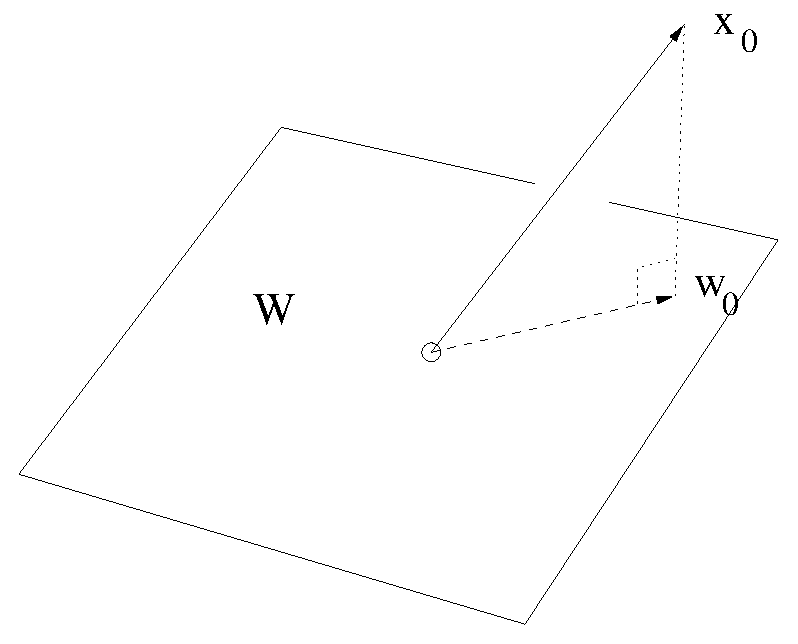
\psfig{file=figures/nearest.eps,width=2.5in}}
        \caption{Approximation of $x_0$ by $w_0\in W$ by least squares.}
        \label{F:nearest}
\end{figure}


The distance between two vectors\index{distance!between vectors}
$v$ and $w$ is $||v-w||$ and the geometric
problem can be rephrased as follows: find a vector $w_0\in W$ such that
\begin{equation}  \label{E:leastsq}
||x_0-w_0||\leq ||x_0-w|| \quad \forall w\in W.
\end{equation}
Condition \Ref{E:leastsq} is called the
{\em least squares approximation}\index{least squares!approximation}.
In order to see where this name comes from we write\Ref{E:leastsq} in the
equivalent form
\[
||x_0-w_0||^2\leq ||x_0-w||^2 \quad \forall w\in W.
\]
This form means that for $w=w_0$ the sum of the squares of the
components of the vector $x_0-w$ is minimal.

Before continuing, we state and prove the {\em Law of Phythagorus\/}.
\index{Law of Phythagorus}  Let $z_1,z_2\in\R^n$ be orthogonal vectors.  Then 
\begin{equation} \label{E:LP}
||z_1+z_2||^2 = ||z_1||^2 + ||z_2||^2.
\end{equation}
To verify \Ref{E:LP} calculate 
\[
||z_1+z_2||^2=(z_1+z_2)\cdot(z_1+z_2)=z_1\cdot z_1 +2z_1\cdot z_2+z_2\cdot z_2
=||z_1||^2 + 2z_1\cdot z_2 +||z_2||^2.
\]
Since $z_1$ and $z_2$ are orthogonal, $z_1\cdot z_2=0$ and the Law of 
Phythagorus is valid.

Using \Ref{E:leastsq} and \Ref{E:LP}, we can rephrase the minimum distance 
problem as follows.
\begin{lemma}  \label{L:orthoLSA}
The vector $w_0\in W$ is the closest vector to $x_0\in\R^n$ if the vector 
$x_0-w_0$ is orthogonal to every vector in $W$. (See Figure~\ref{F:nearest}.)
\end{lemma}

\begin{proof}  Write $x_0-w=z_1+z_2$ where $z_1=x_0-w_0$ and $z_2=w_0-w$.  By 
assumption, $x_0-w_0$ is orthogonal to every vector in $W$; so $z_1$ and 
$z_2\in W$ are orthogonal.  It follows from \Ref{E:LP} that
\[
||x_0-w||^2 = ||x_0-w_0||^2 + ||w_0-w||^2.
\]
Since $||w_0-w||^2\ge 0$, \Ref{E:leastsq} is valid, and $w_0$ is the vector 
nearest to $x_0$ in $W$. \end{proof}

\subsubsection*{Least Squares Distance to a Line}
\index{least squares!distance to a line}
\index{distance!to a line}

Suppose $W$ is as simple a subspace as possible; that is, suppose $W$ is one
dimensional with basis vector $w$.  Since $W$ is one dimensional, a vector
$w_0\in W$ that is closest to $x_0$ must be a multiple of $w$; that is,
$w_0=aw$.  Suppose that we can find a scalar $a$ so that $x_0-aw$ is
orthogonal to every vector in $W$.  Then it follows from
Lemma~\ref{L:orthoLSA} that $w_0$ is the closest vector in $W$ to $x_0$.
To find $a$, calculate
\[
0 = (x_0-aw)\cdot w = x_0\cdot w - a w\cdot w.
\]
Then
\[
a = \frac{x_0\cdot w}{||w||^2}
\]
and
\begin{equation}  \label{E:singleortho}
w_0 = \frac{x_0\cdot w}{||w||^2} w.
\end{equation}
Observe that $||w||^2\not=0$ since $w$ is a basis vector.

For example, if $x_0=(1,2,-1,3)\in\R^4$ and $w=(0,1,2,3)$.  The the vector
$w_0$ in the space spanned by $w$ that is nearest to $x_0$ is
\[
w_0 = \frac{9}{14}w
\]
since $x_0\cdot w=9$ and $||w||^2=14$.

\subsubsection*{Least Squares Distance to a Subspace}
\index{least squares!distance to a subspace}
\index{distance!to a subspace}

Similarly, using Lemma~\ref{L:orthoLSA} we can solve the general least
squares problem by solving a system of linear equations.  Let
$w_1,\ldots,w_k$ be a basis for $W$ and suppose that
\[
w_0 = \alpha_1w_1 + \cdots + \alpha_kw_k
\]
for some scalars $\alpha_i$.  We now show how to find these scalars.

\begin{thm}  \label{T:nearestvector}
Let $x_0\in\R^n$ be a vector, and let $\{w_1,\ldots,w_k\}$ be a
basis\index{basis} for the subspace\index{subspace} $W\subset\R^n$.
Then
\[
w_0 = \alpha_1w_1 + \cdots + \alpha_kw_k
\]
is the nearest vector in $W$ to $x_0$ when
\begin{equation}  \label{E:nearestvector}
\left(\begin{array}{c} \alpha_1 \\ \vdots \\ \alpha_k \end{array}\right) =
(A^tA)\inv A^tx_0,
\end{equation}
where $A=(w_1|\cdots|w_k)$ is the $n\times k$ matrix whose columns are the
basis vectors of $W$.
\end{thm}

\begin{proof} Observe that the vector $x_0-w_0$ is orthogonal to every vector in $W$
precisely when $x_0-w_0$ is orthogonal to each basis vector $w_j$.  It
follows from Lemma~\ref{L:orthoLSA} that $w_0$ is the closest vector to $x_0$
in $W$ if
\[
(x_0-w_0)\cdot w_j = 0
\]
for every $j$.  That is, if
\[
w_0\cdot w_j = x_0\cdot w_j
\]
for every $j$.  These equations can be rewritten as a system of equations in
terms of the $\alpha_i$, as follows:
\begin{equation}  \label{E:dots}
 \begin{array}{ccc}
w_1\cdot w_1\alpha_1 + \cdots + w_1\cdot w_k\alpha_k & = & w_1\cdot x_0\\
 & \vdots &  \\
w_k\cdot w_1\alpha_1 + \cdots + w_k\cdot w_k\alpha_k & = & w_k\cdot x_0.
\end{array}
\end{equation}

Note that if $u,v\in\R^n$ are column vectors, then $u\cdot v= u^tv$. Therefore,
we can rewrite \Ref{E:dots} as
\[
A^tA \left(\begin{array}{c} \alpha_1\\ \vdots \\ \alpha_k \end{array}\right) =
A^tx_0,
\]
where $A$ is the matrix whose columns are the $w_j$ and $x_0$ is viewed as a
column vector.  Note that the matrix $A^tA$ is a $k\times k$ matrix.

We claim that $A^tA$ is invertible.  To verify this claim, it suffices to
show that the null space\index{null space}
of $A^tA$ is zero; that is, if $A^tA z = 0$ for some
$z\in\R^k$, then $z=0$.  First, calculate
\[
||Az||^2 = Az\cdot Az = (Az)^tAz = z^tA^tAz= z^t0 = 0.
\]
It follows that $Az=0$.  Now if we let $z=(z_1,\ldots,z_k)^t$, then the
equation $Az=0$ may be rewritten as
\[
z_1w_1 + \cdots + z_kw_k = 0.
\]
Since the $w_j$ are linearly independent, it follows that the $z_j=0$.  In
particular, $z=0$.  Since $A^tA$ is invertible, \Ref{E:nearestvector} is
valid, and the theorem is proved. \end{proof}


\subsection*{Gram-Schmidt Orthonormalization Process}
\index{Gram-Schmidt orthonormalization}

Suppose that ${\cal W} = \{w_1,\ldots,w_k\}$ is a basis for the subspace
$V\subset\R^n$.  There is a natural process by which the ${\cal W}$ basis
can be transformed into an
orthonormal basis\index{basis!orthonormal}
${\cal V}$ of $V$.  This
process proceeds inductively on the $w_j$; the orthonormal vectors
$v_1,\ldots,v_k$ can be chosen so that
\[
\Span\{v_1,\ldots,v_j\} = \Span\{w_1,\ldots,w_j\}
\]
\index{span}
for each $j\leq k$.  Moreover, the $v_j$ are chosen using the theory of
least squares that we have just discussed.

\subsubsection*{The Case $j=2$}

To gain a feeling for how the induction process works, we verify the case
$j=2$.  Set
\begin{equation}  \label{E:ortho1}
v_1 = \frac{1}{||w_1||}w_1;
\end{equation}
so $v_1$ points in the same direction as $w_1$ and has unit length, that is,
$v_1\cdot v_1=1$.  The normalization is shown in Figure~\ref{F:gram}.

\begin{figure}[htb]
        \centerline{%
        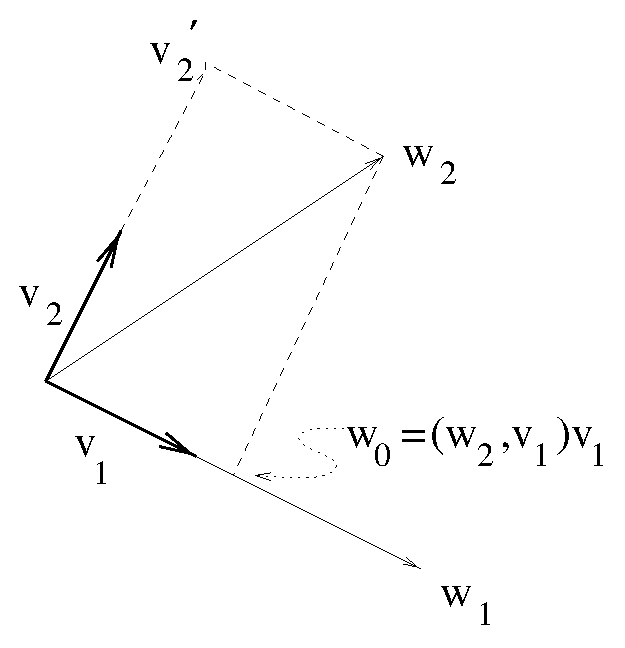
\psfig{file=figures/gram.eps,width=2.0in}}
        \caption{Planar illustration of Gram-Schmidt orthonormalization.}
        \label{F:gram}
\end{figure}

Next, we find a unit length vector $v'_2$ in the plane spanned by $w_1$ and
$w_2$ that is perpendicular\index{perpendicular}
to $v_1$. Let $w_0$ be the vector on the line
generated by $v_1$ that is nearest to $w_2$.  It follows from
\Ref{E:singleortho} that
\[
w_0 = \frac{w_2\cdot v_1}{||v_1||^2}v_1 = (w_2\cdot v_1) v_1.
\]
The vector $w_0$ is shown on Figure~\ref{F:gram} and, as
Lemma~\ref{L:orthoLSA} states, the vector $v_2'=w_2-w_0$ is perpendicular to
$v_1$. That is,
\begin{equation}  \label{E:ortho2}
v'_2 = w_2 - (w_2\cdot v_1) v_1
\end{equation}
is orthogonal\index{orthogonal} to $v_1$.

Finally, set
\begin{equation}  \label{E:ortho3}
v_2 = \frac{1}{||v'_2||}v'_2
\end{equation}
so that $v_2$ has unit length.  Since $v_2$ and $v'_2$ point in the
same direction, $v_1$ and $v_2$ are orthogonal.  Note also that $v_1$ and
$v_2$ are linear combinations of $w_1$ and $w_2$.  Since $v_1$ and $v_2$ are
orthogonal, they are linearly independent.  It follows that
\[
\Span\{v_1,v_2\} = \Span\{w_1,w_2\}.
\]

In summary: computing $v_1$ and $v_2$ using \Ref{E:ortho1}, \Ref{E:ortho2}
and \Ref{E:ortho3} yields an orthonormal basis for the
plane\index{plane} spanned by $w_1$ and $w_2$.

\subsubsection*{The General Case}

\begin{thm} (Gram-Schmidt Orthonormalization) \label{T:orthobasis}
Let $w_1,\ldots,w_k$ be a basis for the subspace $W\subset\R^n$.  Define
$v_1$ as in \Ref{E:ortho1} and then define inductively
\begin{eqnarray}
v'_{j+1} & = & w_{j+1} -(w_{j+1}\cdot v_1)v_1- \cdots -(w_{j+1}\cdot v_j)v_j
\label{E:inductiveGS} \\
v_{j+1} & = & \frac{1}{||v'_{j+1}||}v'_{j+1}. \label{eq:gsnormal}
\end{eqnarray}
Then $v_1,\ldots,v_k$ is an orthonormal basis of $W$ such that for each $j$
\[
\Span\{v_1,\ldots,v_j\} = \Span\{w_1,\ldots,w_j\}
\]
\end{thm}\index{Gram-Schmidt orthonormalization}
\index{basis!orthonormal}

\begin{proof}  We assume that we have constructed orthonormal vectors $v_1,\ldots,v_j$
such that
\[
\Span\{v_1,\ldots,v_j\} = \Span\{w_1,\ldots,w_j\}.
\]
Our purpose is to find a unit vector $v_{j+1}$ that is orthogonal to each $v_i$
and that satisfies
\[
\Span\{v_1,\ldots,v_{j+1}\} = \Span\{w_1,\ldots,w_{j+1}\}.
\]
We construct $v_{j+1}$ in two steps.  First we find a vector $v'_{j+1}$
that is orthogonal to each of the $v_i$ using least squares.  Let $w_0$
be the vector in $\Span\{v_1,\ldots,v_j\}$ that is nearest to $w_{j+1}$.
Theorem~\ref{T:nearestvector} tells us how to make this construction.
Let $A$ be the matrix whose columns are $v_1,\ldots,v_j$.  Then
\Ref{E:nearestvector} states that the coordinates of $w_0$ in the $v_i$ basis
is given by $(A^tA)\inv A^tw_{j+1}$. But since the $v_i$'s are orthonormal,
the matrix $A^tA$ is just $I_k$.  Hence
\[
w_0 =  (w_{j+1}\cdot v_1)v_1 + \cdots + (w_{j+1}\cdot v_j)v_j.
\]
Note that $v'_{j+1}=w_{j+1}-w_0$ is the vector defined in \Ref{E:inductiveGS}.
We claim that $v'_{j+1}=w_{j+1}-w_0$ is orthogonal to $v_k$ for $k\leq j$
and hence to every vector in $\Span\{v_1,\ldots,v_j\}$.  Just calculate
\[
v_{j+1}'\cdot v_k = w_{j+1}\cdot v_k - w_0\cdot v_k =
w_{j+1}\cdot v_k -  w_{j+1}\cdot v_k = 0.
\]
Define $v_{j+1}$ as in
\Ref{eq:gsnormal}.  It follows that $v_1,\ldots,v_{j+1}$ are orthonormal and
that each vector is a linear combination of $w_1,\ldots,w_{j+1}$.  \end{proof}


\subsubsection*{An Example of Orthonormalization}

Let $W\subset\R^4$ be the subspace spanned by the vectors
\begin{equation}  \label{eq:gsexam}
w_1=(1,0,-1,0),\quad w_2=(2,-1,0,1),\quad w_3=(0,0,-2,1).
\end{equation}
We find an orthonormal basis for $W$ using Gram-Schmidt orthonormalization.

\begin{itemize}
\item[Step 1:]   Set
\[
v_1 = \frac{1}{||w_1||}w_1=\frac{1}{\sqrt{2}}(1,0,-1,0).
\]
\item[Step 2:] Following the Gram-Schmidt process, use \Ref{E:inductiveGS} to
define
\[
v'_2 = w_2-(w_2\cdot v_1)v_1= (2,-1,0,1)-\sqrt{2}\frac{1}{\sqrt{2}}(1,0,-1,0)
=(1,-1,1,1).
\]
Normalization using \Ref{eq:gsnormal} yields
\[
v_2 = \frac{1}{||v'_2||}v'_2 = \frac{1}{2}(1,-1,1,1).
\]
\item[Step 3:] Using \Ref{E:inductiveGS} set
\begin{eqnarray*}
v'_3 &=& w_3-(w_3\cdot v_1)v_1-(w_3\cdot v_2)v_2\\
&=&(0,0,-2,1) - \sqrt{2}\frac{1}{\sqrt{2}}(1,0,-1,0)
-\left(-\frac{1}{2}\right)\frac{1}{2}(1,-1,1,1)\\
&=&\frac{1}{4}(-3,-1,-3,5).
\end{eqnarray*}
Normalization using \Ref{eq:gsnormal} yields
\[
v_3 = \frac{1}{||v'_3||}v'_3 = \frac{4}{\sqrt{44}}(-3,-1,-3,5).
\]
\end{itemize}

Hence we have constructed an orthonormal basis $\{v_1,v_2,v_3\}$ for $W$,
namely
\begin{equation}
\label{eq:gsoresult}
\begin{array}{rcccl}
v_1 & = & \frac{1}{\sqrt{2}}(1,0,-1,0) & \approx & (0.7071,0,-0.7071,0)\\
v_2 & = & \frac{1}{2}(1,-1,1,1) & = & (0.5,-0.5,0.5,0.5)\\
v_3 & = & \frac{4}{\sqrt{44}}(-3,-1,-3,5) & \approx &
(-0.4523,-0.1508,-0.4523,0.7538)
\end{array}
\end{equation}


\EXER

\TEXER

\begin{exercise} \label{c7.5.1}
Find an orthonormal basis of $\R^2$ by applying Gram-Schmidt
orthonormalization to the vectors $w_1=(3,4)$ and $w_2=(1,5)$.
\end{exercise}

\begin{exercise} \label{c7.5.2}
Find an orthonormal basis of the plane $W\subset\R^3$ spanned by the
vectors $w_1=(1,2,3)$ and $w_2=(2,5,-1)$ by applying Gram-Schmidt
orthonormalization.
\end{exercise}

\begin{exercise} \label{c7.5.3}
Let ${\cal W}=\{w_1,\ldots,w_k\}$ be an orthonormal basis of the subspace
$W\subset\R^n$.  Prove that ${\cal W}$ can be extended to an orthonormal
basis $\{w_1,\ldots,w_n\}$ of $\R^n$.
\end{exercise}

\CEXER

\begin{exercise} \label{c7.5.4}
Use Gram-Schmidt orthonormalization to find an orthonormal basis for the
subspace of $\R^5$ spanned by the vectors
\begin{equation*}
w1 = (2,1,3,5,7) \quad w2 = (2,-1,5,2,3) \AND w3 = (10,1,-23,2,3).
\end{equation*}
Extend this basis to an orthonormal basis of $\R^5$.
\end{exercise}




\section{Least Squares Fitting of Data} \label{S:7.6}
\index{least squares!fitting of data}
\index{fitting of data}

We begin this section by using the method of least squares to find the
best straight line fit to a set of data.  Later in the section we will
discuss best fits to other curves.

\subsubsection*{An Example of Best Linear Fit to Data}
\index{linear!fit to data}

Suppose that we are given $n$ data points\index{data points}
$(x_i,y_i)$ for $i=1,\ldots,10$.
For example, consider the ten points
\begin{equation*}  \label{E:scatterdata}
\begin{array}{ccccc}
(2.0,0.1) & (3.0,2.7) & (1.5,-1.1) & (-1.0,-5.5) & (0.0,-3.4)\\
(3.6,3.0) & (0.7,-2.8) & (4.1,4.0) & (1.9,-1.9) & (5.0,5.5) \end{array}
\end{equation*}
The ten points $(x_i,y_i)$ are plotted in Figure~\ref{F:linreg} using the
commands
\begin{verbatim}
e10_3_1
plot(X,Y,'o')
axis([-3,7,-8,8])
xlabel('x')
ylabel('y')
\end{verbatim}
\begin{figure}[htb]
     \centerline{%
     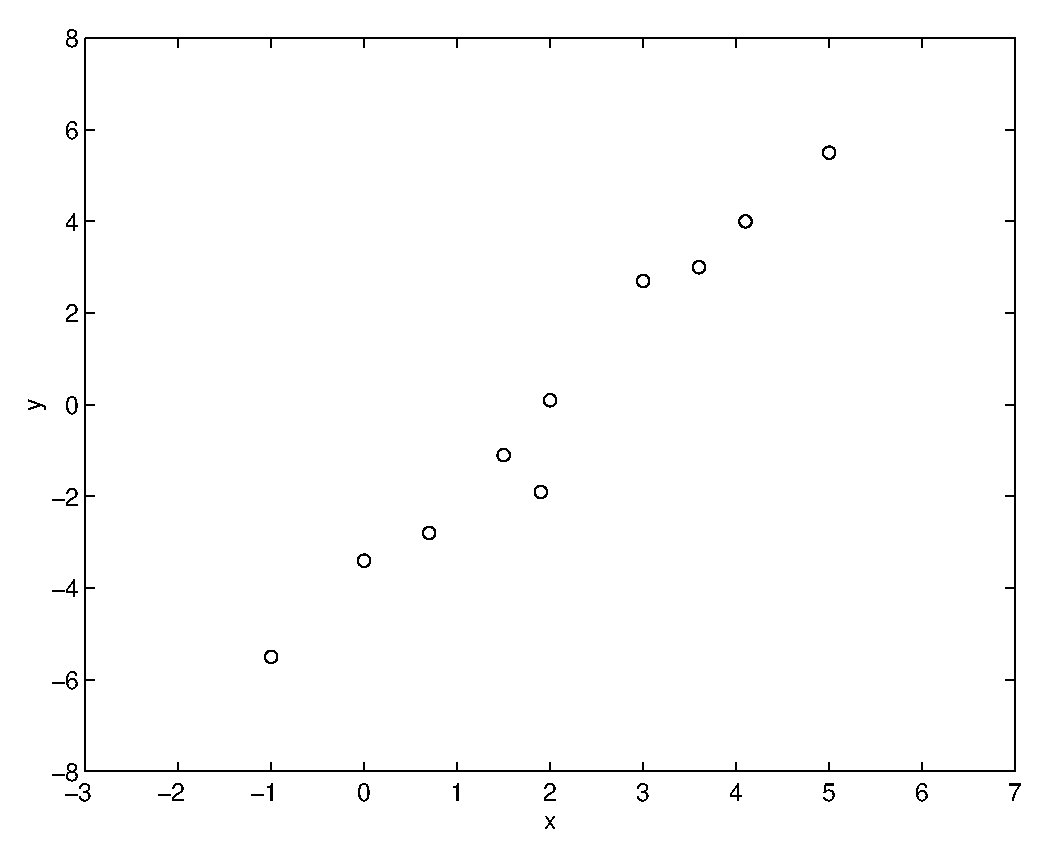
\psfig{file=figures/linreg.eps,width=2.5in}}
     \caption{Scatter plot of data in \protect\Ref{E:scatterdata}.}
     \label{F:linreg}
\end{figure}

Next, suppose that there is a linear relation between the $x_i$ and the $y_i$;
that is, we assume that there are constants $b_1$ and $b_2$ (that do not
depend on $i$) for which $y_i=b_1+b_2x_i$ for each $i$. But these points are
just data; errors may have been made in their measurement.  So we ask:  Find
$b_1^0$ and $b_2^0$ so that the error made in fitting the data to the line
$y=b_1^0+b_2^0x$ is minimal, that is, the error that is made in that fit is
less than or equal to the error made in fitting the data to the line
$y=b_1+b_2x$ for any other choice of $b_1$ and $b_2$.

We begin by discussing what that error actually is.  Given constants $b_1$ and
$b_2$ and given a data point $x_i$, the difference between the
data value\index{data value}
$y_i$ and the hypothesized value $b_1+b_2x_i$ is the error that is made at that
data point.  Next, we combine the errors made at all of the data points; a
standard way to combine the errors is to use the
Euclidean distance\index{distance!Euclidean}
\[
E(b) =
\left((y_1-(b_1+b_2x_1))^2+\cdots+(y_{10}-(b_1+b_2x_{10}))^2\right)^{\half}.
\]
Rewriting $E(b)$ in vector notation leads to an economy in notation and
to a conceptual advantage.  Let
\[
X=(x_1,\ldots,x_{10})^t \quad Y=(y_1,\ldots,y_{10})^t \AND
F_1=(1,1,\ldots,1)
\]
be vectors in $\R^{10}$.  Then in coordinates
\[
Y-(b_1F_1+b_2X) = \left(\begin{array}{c} y_1-(b_1+b_2x_1)\\ \vdots\\
y_{10}-(b_1+b_2x_{10})\end{array}\right).
\]
It follows that
\[
E(b) = ||Y-(b_1F_1+b_2X)||.
\]
The problem of making a least squares fit is to minimize $E$ over all $b_1$
and $b_2$.

To solve the minimization problem\index{minimization problem},
note that the vectors $b_1F_1+b_2X$ form
a two dimensional subspace $W=\Span\{F_1,X\}\subset\R^{10}$
\index{span} (at least when $X$
is not a scalar multiple of $F_1$, which is almost always).  Minimizing $E$ is
identical to finding a vector $w_0=b_1^0F_1+b_2^0X\in W$ that is nearest to
the vector $Y\in\R^{10}$.   This is the
least squares\index{least squares} question that we solved
in the Section~\ref{S:LSA}.

We can use \Matlab to compute the values of $b_1^0$ and $b_2^0$ that give the
best linear approximation to $Y$.  If we set the matrix $A=(F_1|X)$, then
Theorem~\ref{T:nearestvector} implies that the values of $b_1^0$ and $b_2^0$
are obtained using \Ref{E:nearestvector}.  In particular, type {\tt e10\_3\_1}
to call the vectors {\tt X, Y, F1} into \Matlabp, and then type
\begin{verbatim}
A = [F1 X];
b0 = inv(A'*A)*A'*Y
\end{verbatim}
to obtain
\begin{verbatim}
b0(1) = -3.8597
b0(2) =  1.8845
\end{verbatim}
Superimposing the line $y=-3.8597+1.8845x$ on the
scatter plot\index{scatter plot} in
Figure~\ref{F:linreg} yields the plot in Figure~\ref{F:linreg2}.
The total error is $E(b0)=1.9634$ (obtained in \Matlab by typing
{\tt norm(Y-(b0(1)*F1+b0(2)*X)})\index{\computer!norm}.
Compare this with the error
$E(2,-4)=2.0928$.
\begin{figure}[htb]
     \centerline{%
     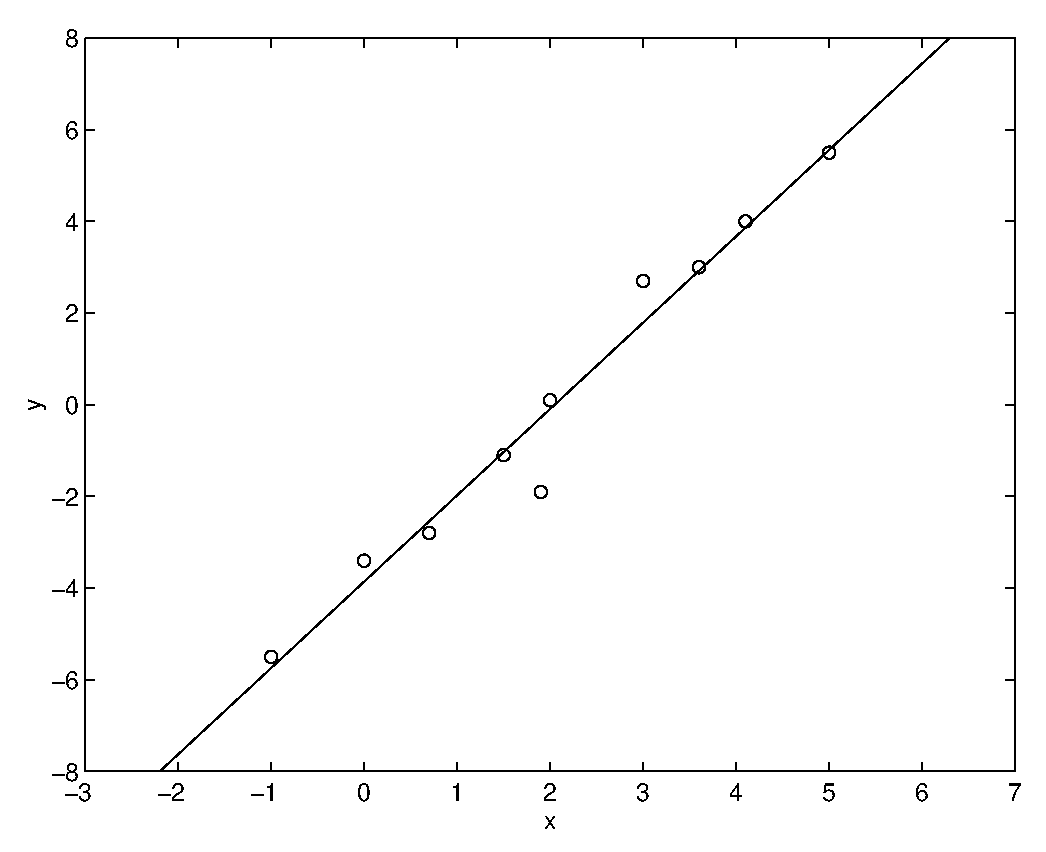
\psfig{file=figures/linreg2.eps,width=2.5in}}
     \caption{Scatter plot of data in \protect\Ref{E:scatterdata} with best
	linear approximation.}
     \label{F:linreg2}
\end{figure}

\subsubsection*{General Linear Regression}
\index{linear!regression}

We can summarize the previous discussion, as follows.  Given $n$ data points
\[
(x_1,y_1),\ldots, (x_n,y_n);
\]
form the vectors
\[
X=(x_1,\ldots,x_n)^t \quad Y=(y_1,\ldots,y_n)^t \AND F_1=(1,\ldots,1)^t
\]
in $\R^n$.  Find constants $b_1^0$ and $b_2^0$ so that $b_1^0F_1+b_2^0X$ is
a vector in $W=\Span\{F_1,X\}\subset\R^n$ that is nearest to $Y$.  Let
\[
A=(F_1|X)
\]
be the $n\times 2$ matrix.  This problem is solved by least squares in
\Ref{E:nearestvector} as
\begin{equation}  \label{E:LSlinfit}
\vectwo{b_1^0}{b_2^0} = (A^tA)\inv A^tY.
\end{equation}


\subsection*{Least Squares Fit to a Quadratic Polynomial}
\index{least squares!fit to a quadratic polynomial}

Suppose that we want to fit the data $(x_i,y_i)$ to a quadratic polynomial
\[
y=b_1+b_2x+b_3x^2
\]
by least squares methods.  We want to find constants $b_1^0,b_2^0,b_3^0$ so
that the error made is using the quadratic polynomial $y=b_1^0+b_2^0x+b_3^0x^2$
is minimal among all possible choices of quadratic polynomials.  The least
squares error is
\[
E(b) = ||Y-\left(b_1F_1+b_2X+b_3X^{(2)}\right)||
\]
where
\[
X^{(2)}=\left(x_1^2,\ldots,x_n^2\right)^t
\]
and, as before, $F_1$ is the $n$ vector with all components equal to $1$.

We solve the minimization problem as before.  In this case, the space of
possible approximations to the data $W$ is three dimensional; indeed,
$W=\Span\{F_1,X,X^{(2)}\}$.  As in the case of fits to lines we try to
find a point in $W$ that is nearest to the vector $Y\in\R^n$.  By
\Ref{E:nearestvector}, the answer is:
\[
b = (A^tA)\inv A^tY,
\]
where $A=(F_1|X|X^{(2)})$ is an $n\times 3$ matrix.

Suppose that we try to fit the data in \Ref{E:scatterdata} with a quadratic
polynomial rather than a linear one.   Use \Matlab as follows
\begin{verbatim}
e10_3_1
A = [F1 X X.*X];
b = inv(A'*A)*A'*Y;
\end{verbatim}
to obtain
\begin{verbatim}
b0(1) =   0.0443
b0(2) =   1.7054
b0(3) =  -3.8197
\end{verbatim}
So the best parabolic fit\index{parabolic fit}
to this data is $y=-3.8197+1.7054x+0.0443x^2$.
Note that the coefficient of $x^2$ is small suggesting that the data was
well fit by a straight line.  Note also that the error is
$E(b0)=1.9098$ which
is only marginally smaller than the error for the best linear fit.  For
comparison, in Figure~\ref{F:linreg3} we superimpose the equation for the
quadratic fit onto Figure~\ref{F:linreg2}.
\begin{figure}[htb]
     \centerline{%
     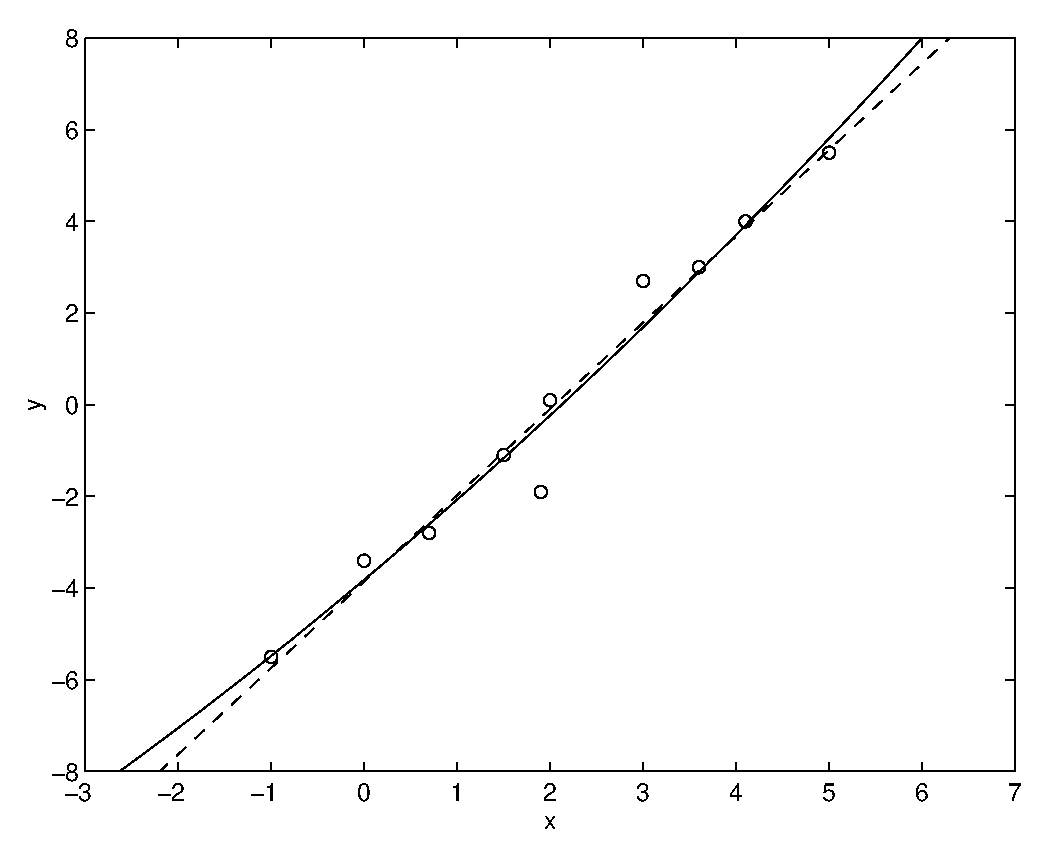
\psfig{file=figures/linreg3.eps,width=2.5in}}
     \caption{Scatter plot of data in \protect\Ref{E:scatterdata} with best
	linear and quadratic approximations.  The best linear fit is plotted
	with a dashed line.}
     \label{F:linreg3}
\end{figure}\index{scatter plot}



\subsection*{General Least Squares Fit}
\index{least squares!general fit}

The approximation to a quadratic polynomial shows that least squares
fits can be made to any finite dimensional
function space\index{function space}.  More precisely,
Let ${\cal C}$ be a finite dimensional space of functions and let
\[
f_1(x),\ldots,f_m(x)
\]
be a basis for ${\cal C}$.  We have just considered two such spaces:
${\cal C}=\Span\{f_1(x)=1,f_2(x)=x\}$ for
linear regression\index{linear!regression} and
${\cal C}=\Span\{f_1(x)=1,f_2(x)=x,f_3(x)=x^2\}$ for
least squares fit to a
quadratic polynomial\index{least squares!fit to a quadratic polynomial}.

The general least squares fit of a data set
\[
(x_1,y_1),\ldots, (x_n,y_n)
\]
is the function $g_0(x)\in{\cal C}$ that is nearest to the data set in the
following sense.  Let
\[
X = (x_1,\ldots,x_n)^t \AND Y = (y_1,\ldots,y_n)^t
\]
be column vectors in $\R^n$.  For any function $g(x)$ define the column vector
\[
G = (g(x_1),\ldots,g(x_n))^t\in\R^n.
\]
So $G$ is the evaluation of $g(x)$ on the data set.  Then the error
\[
E(g) = ||Y-G||
\]
is minimal for $g=g_0$.

More precisely, we think of the data $Y$ as representing the (approximate)
evaluation of a function on the $x_i$.  Then we try to find a function
$g_0\in{\cal C}$ whose values on the $x_i$ are as near as possible to
the vector $Y$.  This is just a least squares problem.  Let $W\subset\R^n$ be
the vector subspace spanned by the evaluations of function $g\in{\cal C}$ on
the data points $x_i$, that is, the vectors $G$.  The minimization problem
is to find a vector in $W$ that is nearest to $Y$.  This can be solved in
general using \Ref{E:nearestvector}.  That is, let $A$ be the $n\times m$
matrix
\[
A = (F_1|\cdots|F_m)
\]
where $F_j\in\R^n$ is the column vector associated to the $j^{th}$ basis
element of ${\cal C}$, that is,
\[
F_j = (f_j(x_1),\ldots,f_j(x_n))^t\in\R^n.
\]
The minimizing function $g_0(x)\in{\cal C}$ is a linear combination of the
basis functions $f_1(x),\ldots,f_n(x)$, that is,
\[
g_0(x) = b_1f_1(x) + \cdots + b_mf_m(x)
\]
for scalars $b_i$.  If we set
\[
b = (b_1,\ldots,b_m)\in\R^m,
\]
then least squares minimization states that
\begin{equation}  \label{E:LSFG}
b = (A'A)\inv A'Y.
\end{equation}

This equation can be solved easily in \Matlabp.  Enter the data as column
$n$-vectors {\tt X} and {\tt Y}.  Compute the column vectors
{\tt Fj = $f_j$(X)} and then form the matrix {\tt A = [F1 F2 $\cdots$ Fm]}.
Finally compute
\begin{verbatim}
b = inv(A'*A)*A'*Y
\end{verbatim}


\subsubsection*{Least Squares Fit to a Sinusoidal Function}
\index{least squares!fit to a sinusoidal function}

We discuss a specific example of the general least squares formulation by
considering the weather.  It is reasonable to expect monthly data on the
weather to vary periodically in time with a period of one year.  In
Table~\ref{T:parrio} we give average daily high and low temperatures for
each month of the year for Paris and Rio de Janeiro.  We attempt to fit this
data with curves of the form:
\[
g(T) = b_1 + b_2\cos\left(\frac{2\pi}{12}T\right) +
b_3\sin\left(\frac{2\pi}{12}T\right),
\]
where $T$ is time measured in months and $b_1,b_2,b_3$ are scalars.  These
functions are $12$ periodic, which seems appropriate for weather data, and
form a three dimensional function space ${\cal C}$.  Recall the trigonometric
identity
\[
a\cos(\omega t) + c\sin(\omega t) = d\sin(\omega(t-\varphi))
\]
where
\[
d = \sqrt{a^2+c^2}.
\]
Based on this identity we call ${\cal C}$ the space of {\em sinusoidal
functions\/}\index{sinusoidal functions}.  The number $d$ is called
the {\em amplitude\/}\index{amplitude} of the
sinusoidal function $g(T)$.



\begin{table}[htb]
\begin{center}
\begin{tabular}{|c||c|c||c|c|||c||c|c||c|c|}
\hline
  & \multicolumn{2}{c||}{Paris} & \multicolumn{2}{c|||}{Rio de Janeiro} &
  & \multicolumn{2}{c||}{Paris} & \multicolumn{2}{c|}{Rio de Janeiro}\\
Month & High & Low & High & Low & Month & High & Low & High & Low\\
\hline
  1 & 55 & 39 & 84 & 73 &   7 & 81 & 64 & 75 & 63 \\
  2 & 55 & 41 & 85 & 73 &   8 & 81 & 64 & 76 & 64 \\
  3 & 59 & 45 & 83 & 72 &   9 & 77 & 61 & 75 & 65 \\
  4 & 64 & 46 & 80 & 69 &  10 & 70 & 54 & 77 & 66 \\
  5 & 68 & 55 & 77 & 66 &  11 & 63 & 46 & 79 & 68 \\
  6 & 75 & 61 & 76 & 64 &  12 & 55 & 41 & 82 & 71 \\
\hline
\end{tabular}
\caption{Monthly Average of Daily High and Low Temperatures in Paris and Rio de
Janeiro.}
\label{T:parrio}
\end{center}
\end{table}

Note that each data set consists of twelve entries --- one for each month.
Let $T=(1,2,\ldots,12)^t$ be the vector $X\in\R^{12}$ in the general
presentation.  Next let $Y$ be the data in one of the data sets --- say the
high temperatures in Paris.

Now we turn to the vectors representing basis functions in ${\cal C}$.
Let
\begin{verbatim}
F1=[1 1 1 1 1 1 1 1 1 1 1 1]'
\end{verbatim}
be the vector associated with the basis function $f_1(T)=1$. Let  {\tt F2}
and {\tt F3} be the column vectors associated to the basis functions
\[
f_2(T) = \cos\left(\frac{2\pi}{12} T\right) \AND
f_3(T) = \sin\left(\frac{2\pi}{12} T\right).
\]
These vectors are computed by typing
\begin{verbatim}
F2 = cos(2*pi/12*T);
F3 = sin(2*pi/12*T);
\end{verbatim}
By typing {\tt temper}, we enter the temperatures and the vectors {\tt T},
{\tt F1},  {\tt F2} and {\tt F3} into \Matlabp.

To find the best fit to the data by a sinusoidal function $g(T)$, we use
\Ref{E:nearestvector}.  Let $A$ be the $12\times 3$ matrix
\begin{verbatim}
A = [F1 F2 F3];
\end{verbatim}

The table data is entered in column vectors {\tt ParisH} and {\tt ParisL} for
the high and low Paris temperatures and {\tt RioH} and {\tt RioL} for the
high and low Rio de Janeiro temperatures.  We can find the best least squares
fit of the Paris high temperatures by a sinusoidal function $g_0(T)$ by typing
\begin{verbatim}
b = inv(A'*A)*A'*ParisH
\end{verbatim}
obtaining
\begin{verbatim}
b(1) =  66.9167
b(2) =  -9.4745
b(3) =  -9.3688
\end{verbatim}
The result is plotted in Figure~\ref{F:ParisH} by typing
\begin{verbatim}
plot(T,ParisH,'o')
axis([0,13,0,100])
xlabel('time (months)')
ylabel('temperature (Fahrenheit)')
hold on
xx = linspace(0,13);
yy = b(1) + b(2)*cos(2*pi*xx/12) + b(3)*sin(2*pi*xx/12);
plot(xx,yy)
\end{verbatim}

\begin{figure}[htb]
     \centerline{%
     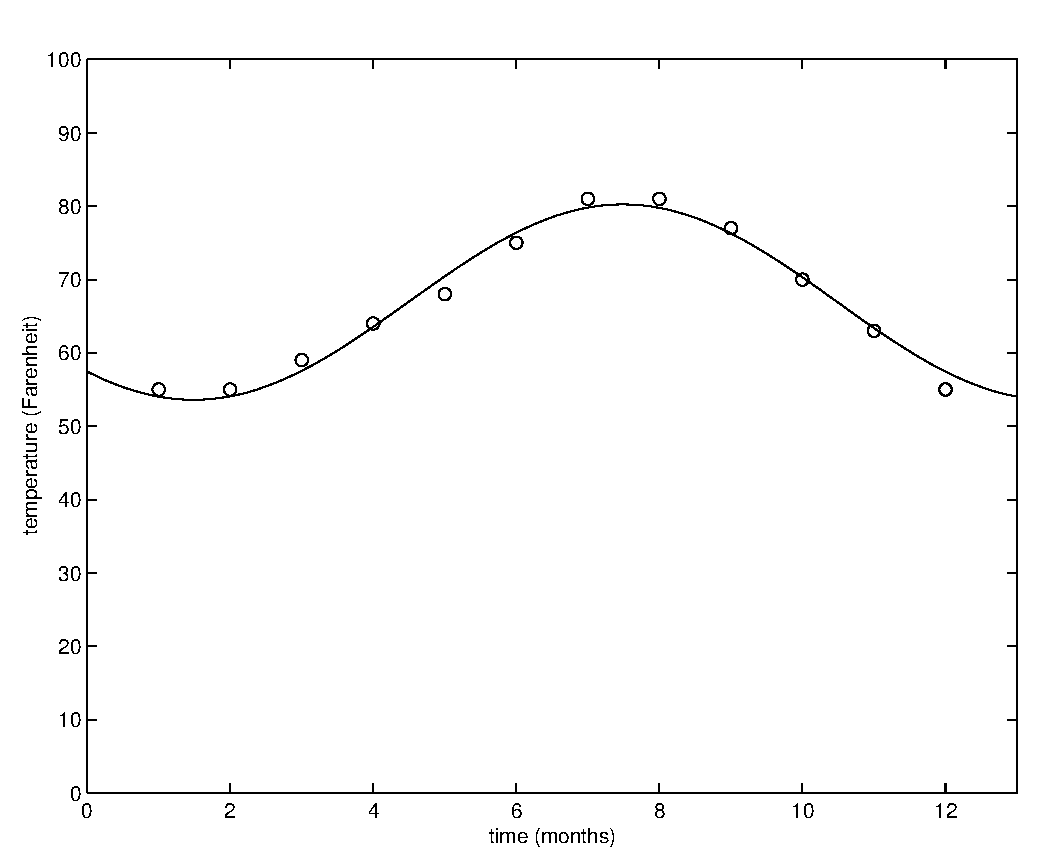
\psfig{file=figures/ParisH.eps,width=2.5in}
     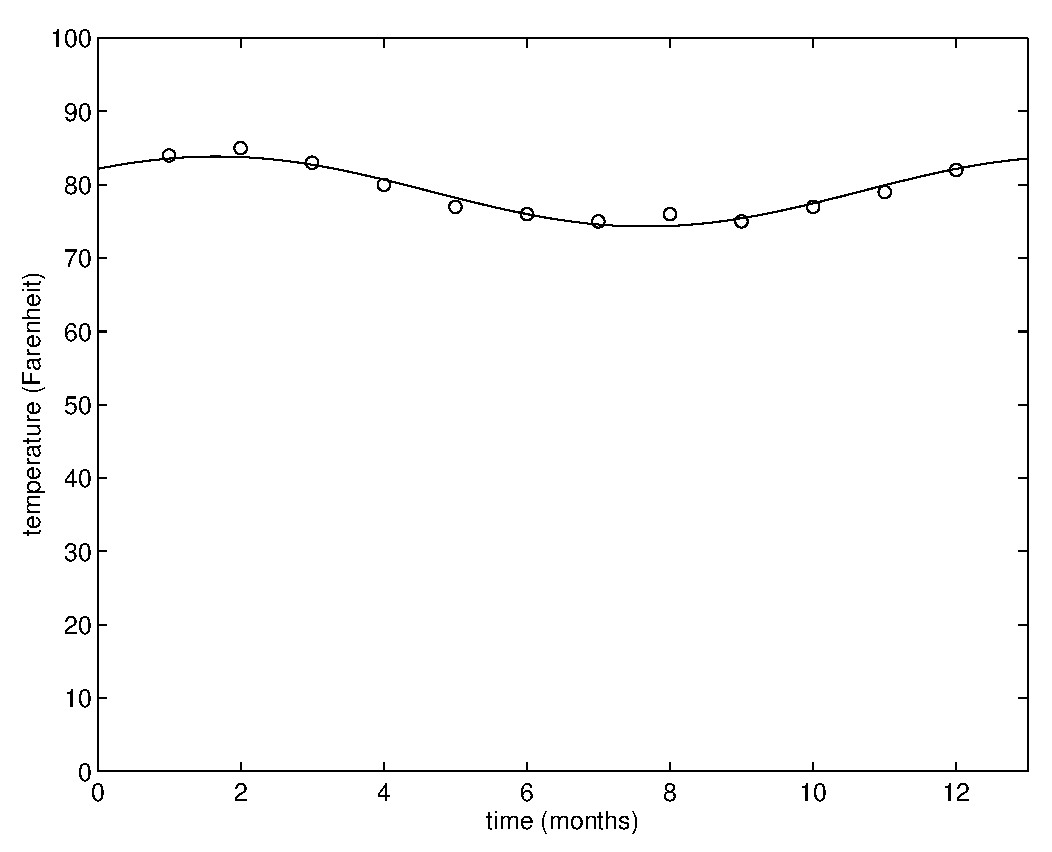
\psfig{file=figures/RioH.eps,width=2.5in}}
     \caption{Monthly averages of daily high temperatures in Paris (left) and
	Rio de Janeiro (right) with best sinusoidal approximation.}
     \label{F:ParisH}
\end{figure}

A similar exercise allows us to compute the best approximation to the
Rio de Janeiro high temperatures obtaining
\begin{verbatim}
b(1) =  79.0833
b(2) =   3.0877
b(3) =   3.6487
\end{verbatim}
The value of $b(1)$ is just the mean high temperature and not surprisingly
that value is much higher in Rio than in Paris.  There is yet more
information contained in these approximations.   For
the high temperatures in Paris and Rio
\[
d_P = 13.3244 \AND d_R = 4.7798.
\]
The amplitude $d$ measures the variation of the high temperature about its
mean.  It is much greater in Paris than in Rio, indicating that the
difference in temperature between winter and summer is much greater in Paris
than in Rio.

\subsubsection*{Least Squares Fit in \Matlabp}

The general formula for a least squares fit of data \Ref{E:LSFG} has been
preprogrammed in \Matlabp.  After setting up the matrix $A$ whose columns are 
the vectors $F_j$ just type
\begin{verbatim}
b = A\Y
\end{verbatim}
This \Matlab command can be checked on the sinusoidal fit to the high 
temperature Rio de Janeiro data by typing
\begin{verbatim}
b = A\RioH
\end{verbatim} 
and obtaining
\begin{verbatim}
b =
   79.0833
    3.0877
    3.6487
\end{verbatim}


\EXER

\CEXER

\begin{exercise} \label{c7.6.1}
World population data for each decade of this century (except for 1910)
is given in Table~\ref{T:popdata}.  Assume that population growth is linear
$P=mT+b$ where time $T$ is measured in decades since the year 1900 and $P$ is
measured in billions of people.  This data can be recovered by typing
{\tt e10\_3\_po}.
\begin{itemize}
\item[(a)]  Find $m$ and $b$ to give the best linear fit to this data.
\item[(b)]  Use this linear approximation to the data to make predictions
of the world populations in the year 1910 and 2000.
\item[(c)]  Do you expect the prediction for the year 2000 to be high or low
or on target? Explain why by graphing the data with the best linear fit
superimposed and by using the differential equation population model
discussed in Section~\ref{S:growthmodels}.
\end{itemize}
\begin{table}[htb]
\begin{center}
\begin{tabular}{|c|c||c|c|}
\hline
Year & Population (in millions) & Year & Population (in millions)\\
\hline
1900 & 1625 & 1950 & 2516  \\
1910 & n.a. & 1960 & 3020 \\
1920 & 1813 & 1970 & 3698 \\
1930 & 1987 & 1980 & 4448 \\
1940 & 2213 & 1990 & 5292 \\
\hline
\end{tabular}
\caption{Twentieth Century World Population Data by Decades.}
\label{T:popdata}
\end{center}
\end{table}

\end{exercise}

\begin{exercise} \label{c7.6.2}
Find the best sinusoidal approximation to the monthly average low temperatures
in Paris and Rio de Janeiro.  How does the variation of these temperatures
about the mean compare to the high temperature calculations?  Was this the
result you expected?
\end{exercise}


\begin{exercise} \label{c7.6.3}
In Table~\ref{T:sunny} we present weather data from ten U.S. cities.  The
data is the average number of days in the year with precipitation and the
percentage of sunny hours to hours when it could be sunny.  Find the best
linear fit to this data.
\begin{table}[htb]
\begin{center}
\begin{tabular}{|c||c|c||c||c|c|}
\hline
City & Rainy Days & Sunny (\%) & City & Rainy Days & Sunny (\%)\\
\hline
Charleston 	&   92 & 72 & Kansas City 	&   98 & 59\\
Chicago 	&  121 & 54 & Miami 		&  114 & 85 \\
Dallas 		&   82 & 65 & New Orleans 	&  103 & 61 \\
Denver 		&   82 & 67 & Phoenix 		&   28 & 88 \\
Duluth 		&  136 & 52 & Salt Lake City 	&   99 & 59 \\
\hline
\end{tabular}
\caption{Precipitation Days Versus Sunny Time for Selected U.S. Cities.}
\label{T:sunny}
\end{center}
\end{table}
\end{exercise}


\section{Symmetric Matrices}
\label{S:symmetric}

Symmetric matrices have some remarkable properties that can be
summarized by:
\begin{thm}  \label{T:symmetricmat}
Let $A$ be an $n\times n$ symmetric matrix\index{matrix!symmetric}.
Then
\begin{enumerate}
\item[(a)] every eigenvalue\index{eigenvalue!of symmetric matrix}
of $A$ is real, and
\item[(b)] there is an orthonormal basis\index{basis!orthonormal}
of $\R^n$ consisting of
	eigenvectors of $A$.
\end{enumerate}
\end{thm}

As a consequence of Theorem~\ref{T:symmetricmat}, let
${\cal V}=\{v_1,\ldots,v_n\}$ be an orthonormal basis for $\R^n$
consisting of eigenvectors of $A$.  Indeed, suppose
\[
Av_j = \lambda_jv_j
\]
where $\lambda_j\in\R$.  Note that
\[
Av_j\cdot v_i =  \left\{\begin{array}{rl} \lambda_j & \qquad i=j\\
			0 & \qquad i\neq j \end{array}\right.
\]
It follows from \Ref{e:coordorthomat} that
\[
[A]_{\cal V}= \left(\begin{array}{ccc} \lambda_1 & & 0 \\  & \ddots & \\
	0 &  & \lambda_n \end{array}\right)
\]
is a diagonal matrix.  So every symmetric matrix is similar to a diagonal
matrix.

\subsubsection*{Hermitian Inner Products}

The proof of Theorem~\ref{T:symmetricmat} uses the {\em Hermitian inner
product}\index{Hermitian inner product} --- a generalization of
dot product\index{dot product} to complex vectors\index{vector!complex}.
Let $v,w\in\C^n$ be two complex $n$-vectors.  Define
\[
\langle v,w \rangle = v_1\overline{w}_1 + \cdots + v_n\overline{w}_n.
\]
Note that the coordinates $w_i$ of the second vector enter this formula
with a complex conjugate.  However, if $v$ and $w$ are real vectors, then
\[
\langle v,w \rangle = v\cdot w.
\]
A more compact notation for the Hermitian inner product is given by
matrix multiplication\index{matrix!multiplication}.
Suppose that $v$ and $w$ are column $n$-vectors.
Then
\[
\langle v,w \rangle = v^t\overline{w}.
\]

The properties of the Hermitian inner product are similar to those of dot
product.  We note three.  Let $c\in\C$ be a complex scalar.  Then
\begin{eqnarray*}
\langle v,v \rangle & = & ||v||^2\ge 0\\
\langle cv,w \rangle & = & c\langle v,w \rangle \\
\langle v,cw \rangle & = & \overline{c} \langle v,w \rangle
\end{eqnarray*}
Note the complex conjugation of the complex scalar $c$ in the previous
formula.

Let $C$ be a complex $n\times n$ matrix.  Then the main observation
concerning Hermitian inner products that we shall use is:
\[
\langle Cv,w \rangle = \langle v,\overline{C}^tw \rangle.
\]
This fact is verified by calculating
\[
\langle Cv,w \rangle = (Cv)^t\overline{w} = (v^tC^t)\overline{w}
= v^t(C^t\overline{w}) = v^t(\overline{\overline{C}^tw})
= \langle v,\overline{C}^tw \rangle.
\]
So if $A$ is a $n\times n$ real symmetric matrix, then
\begin{equation}   \label{e:symminv}
\langle Av,w \rangle = \langle v,Aw \rangle,
\end{equation}
since $\overline{A}^t= A^t = A$.

\begin{proof}[Theorem~\ref{T:symmetricmat}(a)]  Let $\lambda$
be an eigenvalue of $A$ and let $v$ be the associated eigenvector. Since
$Av=\lambda v$ we can use \Ref{e:symminv} to compute
\[
\lambda \langle v,v \rangle = \langle Av,v \rangle = \langle v,Av \rangle
= \overline{\lambda} \langle v,v \rangle.
\]
Since $\langle v,v \rangle = ||v||^2 > 0$, it follows that
$\lambda=\overline{\lambda}$ and $\lambda$ is real.  \end{proof}


\begin{proof}[Theorem~\ref{T:symmetricmat}(b)]
Let $A$ be a real symmetric $n\times n$ matrix.  We want to show that there
is an orthonormal basis of $\R^n$ consisting of eigenvectors of $A$.  The
proof proceeds inductively on $n$.   The theorem is trivially valid for
$n=1$; so we assume that it is valid for $n-1$.

Theorem~\ref{T:eigens} of Chapter~\ref{C:D&E} implies that $A$ has an 
eigenvalue $\lambda_1$ and Theorem~\ref{T:symmetricmat}(a) states that 
this eigenvalue is real.
Let $v_1$ be a unit length eigenvector corresponding to the eigenvalue
$\lambda_1$.  Extend $v_1$ to an orthonormal basis $v_1,w_2,\ldots,w_n$ of
$\R^n$ and let $P=(v_1|w_2|\cdots|w_n)$ be the matrix whose columns are the
vectors in this orthonormal basis.  Orthonormality and direct multiplication
implies that
\begin{equation}  \label{e:orthosym}
P^tP=I_n.
\end{equation}
Therefore $P$ is invertible; indeed $P\inv=P^t$.

Next, let
\[
B= P\inv AP.
\]
By direct computation
\[
Be_1 = P\inv APe_1 = P\inv Av_1 = \lambda_1 P\inv v_1=\lambda_1e_1.
\]
It follows that that $B$ has the form
\[
B = \mattwo{\lambda_1}{*}{0}{C}
\]
where $C$ is an $(n-1)\times (n-1)$ matrix.   Since $P\inv=P^t$, it follows
that $B$ is a symmetric matrix; to verify this point compute
\[
B^t = (P^t AP)^t = P^t A^t (P^t)^t = P^tAP = B.
\]
It follows that
\[
B =\mattwo{\lambda_1}{0}{0}{C}
\]
where $C$ is a symmetric matrix.  By induction we can choose an orthonormal
basis $z_2,\ldots,z_n$ in $\{0\}\times\R^{n-1}$ consisting of eigenvectors
of $C$.  It follows that $e_1,z_2,\ldots,z_n$ is an orthonormal basis for
$\R^n$ consisting of eigenvectors of $B$.

Finally, let $v_j=P\inv z_j$ for $j=2,\ldots,n$.  Since $v_1=P\inv e_1$,
it follows that  $v_1,v_2,\ldots,v_n$ is a basis of $\R^n$ consisting of
eigenvectors of $A$.  We need only show that the $v_j$ form an orthonormal
basis of $\R^n$.   This is done using \Ref{e:symminv}.  For notational
convenience let $z_1=e_1$ and compute
\[
\langle v_i,v_j \rangle  =\langle P\inv z_i,P\inv z_j\rangle =
\langle P^tz_i, P^tz_j \rangle = \langle z_i, PP^t z_j \rangle =
\langle z_i,z_j \rangle,
\]
since $PP^t= I_n$.  Thus the vectors $v_j$ form an orthonormal basis since
the vectors $z_j$ form an orthonormal basis.  \end{proof}




\EXER

\TEXER

\begin{exercise} \label{c7.7.1}
Let
\[
A = \mattwo{a}{b}{b}{d}
\]
be the general real $2\times 2$ symmetric matrix.
\begin{itemize}
\item[(a)]  Prove directly using the discriminant of the characteristic
polynomial that $A$ has real eigenvalues.
\item[(b)]  Show that $A$ has equal eigenvalues only if $A$ is a scalar
multiple of $I_2$.
\end{itemize}
\end{exercise}

\begin{exercise} \label{c7.7.2}
Let
\[
A=\mattwo{1}{2}{2}{-2}.
\]
Find the eigenvalues and eigenvectors of $A$ and verify that the eigenvectors
are orthogonal.
\end{exercise}

\CEXER

\noindent In Exercises~\ref{exer:powita} -- \ref{exer:powitc}
compute the eigenvalues and the eigenvectors of the 
$2\times 2$ matrix.  Then load the matrix into the program {\sf map}
\index{\computer!map} in \Matlab and iterate.  That is, choose an initial
vector $v_0$ and use {\sf map} to compute $v_1=Av_0$, $v_2=Av_1$, \ldots.
How does the result of iteration compare with the eigenvectors and
eigenvalues that you have found?
{\bf Hint:} You may find it convenient to use the feature {\sf Rescale} in
the {\sf MAP Options}.  Then the norm of the vectors is rescaled to $1$
after each use of the command {\sf Map} and the vectors $v_j$ will not
escape from the viewing screen.
\begin{exercise}  \label{exer:powita}
$A=\mattwo{1}{3}{3}{1}$
\end{exercise}
\begin{exercise}  \label{exer:powitb}
$B=\mattwo{11}{9}{9}{11}$
\end{exercise}
\begin{exercise}  \label{exer:powitc}
$C=\mattwo{0.005}{-2.005}{-2.005}{0.005}$
\end{exercise}

\begin{exercise} \label{c7.7.3}
Perform the same computational experiment as described in
Exercises~\ref{exer:powita} -- \ref{exer:powitc} using the matrix
$A=\mattwo{0}{2}{2}{0}$
and the program {\sf map}.  How do your results differ from the results
in those exercises and why?
\end{exercise}



\section{Orthogonal Matrices and $QR$ Decompositions}
\label{S:QR}

In this section we describe an alternative approach to Gram-Schmidt
orthonormalization for constructing an orthonormal basis of a subspace
$W\subset\R^n$.  This method is called the $QR$ decomposition and is
numerically
superior to Gram-Schmidt.  Indeed, the $QR$ decomposition is the method used by
\Matlab to compute orthonormal bases.  To discuss this decomposition we need
to introduce a new type of matrices, the orthogonal matrices.

\subsection*{Orthogonal Matrices}

\begin{Def} \label{def:orthmat}
\index{matrix!orthogonal}
An $n\times n$ matrix $Q$ is {\em orthogonal\/} if its columns form an
orthonormal basis\index{basis!orthonormal}
of $\R^n$.
\end{Def}

The following lemma states elementary properties of orthogonal matrices:
\begin{lemma} \label{lem:orthprop}
Let $Q$ be an $n\times n$ matrix.  Then
\begin{itemize}
\item[(a)] $Q$ is orthogonal if and only if $Q^tQ=I_n$;
\item[(b)] $Q$ is orthogonal if and only if $Q^{-1} = Q^t$;
\item[(c)] If $Q_1,Q_2$ are orthogonal matrices, then $Q_1Q_2$ is
an orthogonal matrix.
\end{itemize}
\end{lemma}
\begin{proof}  (a) Let $Q=(v_1|\cdots|v_n)$.  Since $Q$ is orthogonal, the $v_j$
form an orthonormal basis.  By direct computation note that
$Q^tQ=\{(v_i\cdot v_j)\}=I_n$, since the $v_j$ are orthonormal. Note that
(b) is simply a restatement of (a).

\noindent (c) Now let $Q_1,Q_2$ be orthogonal. Then (a) implies
\[
(Q_1Q_2)^t(Q_1Q_2) = Q_2^tQ_1^tQ_1Q_2 = Q_2^tQ_2 = I_n,
\]
thus proving (c).  \end{proof}

The previous lemma together with \Ref{e:orthosym} in the proof of
Theorem~\ref{T:symmetricmat}(b) lead to the following result:
\begin{prop}  For each symmetric $n\times n$ matrix $A$, there exists an
orthogonal matrix $P$ such that $P^tAP$ is a diagonal matrix.
\end{prop}

\subsubsection*{Reflections Across Hyperplanes: Householder Matrices}

Useful examples of orthogonal matrices are reflections across
hyperplanes.  An $n-1$ dimensional subspace of $\R^n$ is called a
{\em hyperplane\/}.\index{hyperplane}  Let $V$ be a hyperplane and let $u$
be a nonzero vector normal to $V$.  Then a
{\em reflection\/}\index{reflection} across $V$ is
a linear map $H:\R^n\to\R^n$ such that
\begin{itemize}
\item[(a)] $Hv=v$ for all $v\in V$.
\item[(b)] $Hu = -u$.
\end{itemize}
We claim that the matrix of a reflection across a hyperplane is orthogonal
and there is a simple formula for that matrix.
\begin{Def} \label{D:Householder}
A {\em Householder matrix\/} is an $n\times n$ matrix of the form
\begin{equation} \label{eq:householder}
H=I_n - \frac{2}{u^tu} u u^t
\end{equation}
where $u\in\R^n$ is a nonzero vector. \index{matrix!Householder}.
\end{Def}
This definition makes sense since $u^tu=||u||^2$ is a number while the
product $u u^t$ is an $n\times n$ matrix.

\begin{lemma}
Let $u\in\R^n$ be a nonzero vector and let $V$ be the hyperplane orthogonal
to $u$.  Then the Householder matrix $H$ is a
reflection\index{reflection} across $V$ and is orthogonal.
\end{lemma}

\begin{proof}
By definition every vector $v\in V$ satisfies $u^tv=u\cdot v =0$.  Therefore,
\[
Hv = v - \frac{2}{u^tu} u u^tv = v,
\]
and
\[
Hu = u - \frac{2}{u^tu} u u^tu =  u-2u = -u.
\]
Hence $H$ is a reflection across the hyperplane $V$.  It also follows that
$H^2=I_n$ since $H^2v = H(Hv) = Hv = v$ for all $v\in V$ and $H^2u=H(-u)=u$.
So $H^2$ acts like the identity on a basis of $\R^n$ and $H^2=I_n$.

To show that $H$ is orthogonal, we first calculate
\[
H^t = I_n^t - \frac{2}{u^tu} (uu^t)^t= I_n - \frac{2}{u^tu}uu^t = H.
\]
Therefore $I_n = H H = HH^t$ and $H^t=H\inv$.  Now apply
Lemma~\ref{lem:orthprop}(b).   \end{proof}

\subsection*{$QR$ Decompositions}

The Gram-Schmidt process is not used in practice to find orthonormal bases
as there are other techniques available that are preferable for
orthogonalization on a computer.  One such procedure for the construction of
an orthonormal basis is based on $QR$ decompositions using {\em Householder
transformations}\index{matrix!Householder}.  This method is the one
implemented in \Matlab.

An $n\times k$ matrix $R=\{r_{ij}\}$ is {\em upper triangular\/} if
$r_{ij}=0$ whenever $i>j$.

\begin{Def}  \label{qr-Def} \index{QR decomposition}
An $n\times k$ matrix $A$ has a {\em $QR$ decomposition\/} if
\begin{equation} \label{eq:qrdecom}
A=QR.
\end{equation}
where $Q$ is an $n\times n$
orthogonal matrix\index{matrix!orthogonal}
and $R$ is an $n\times k$
upper triangular matrix\index{matrix!upper triangular} $R$.
\end{Def}

$QR$ decompositions can be used to find orthonormal bases as follows.
Suppose that ${\cal W} = \{w_1,\ldots,w_k\}$ is a basis for the subspace
$W\subset\R^n$.  Then define the $n\times k$ matrix $A$ which has the $w_j$
as columns, that is
\[
A = (w_1^t|\cdots|w_k^t).
\]
Suppose that $A=QR$ is a $QR$ decomposition.  Since $Q$ is orthogonal, the
columns of $Q$ are orthonormal.  So write
\[
Q = (v_1^t|\cdots|v_n^t).
\]
On taking transposes we arrive at the equation $A^t=R^tQ^t$:
\[
\left(\begin{array}{c} w_1 \\ \vdots \\ w_k \end{array} \right)
= \left(\begin{array}{cccccc}  r_{11} & 0 & \cdots & 0 & \cdots & 0\\
	r_{12} & r_{22} & \cdots & 0  & \cdots & 0 \\
	\vdots & \vdots & \cdots & \vdots & \cdots & \vdots\\
	r_{1k} & r_{2k} & \cdots & r_{kk}& \cdots & 0 \end{array} \right)
 \left(\begin{array}{c} v_1 \\ \vdots \\ v_n \end{array} \right).
\]
By equating rows in this matrix equation we arrive at the system
\begin{equation} \label{eq:wrv}
\begin{array}{rcl}
w_1 & = & r_{11}v_1 \\
w_2 & = & r_{12}v_1 + r_{22}v_2 \\
& \vdots & \\
w_k & = & r_{1k}v_1 + r_{2k}v_2 + \cdots + r_{kk}v_k.
\end{array}
\end{equation}
It now follows that the $W=\Span\{v_1,\ldots,v_k\}$ and that
$\{v_1,\ldots,v_k\}$ is an orthonormal basis for $W$.  We have proved:

\begin{prop} \label{prop:qrdec}
Suppose that there exist an orthogonal $n\times n$ matrix $Q$ and an upper
triangular $n\times k$ matrix $R$ such that the $n\times k$ matrix $A$ has
a $QR$ decomposition\index{QR decomposition}
\[
A=QR.
\]
Then the first $k$ columns $v_1,\ldots,v_k$ of the matrix $Q$ form an
orthonormal basis\index{basis!orthonormal}
of the subspace $W=\Span\{w_1,\ldots,w_k\}$, where the $w_j$
are the columns of $A$.  Moreover, $r_{ij}=v_i\cdot w_j$ is the coordinate
of $w_j$ in the orthonormal basis.
\end{prop}

Conversely, we can also write down a $QR$ decomposition for a matrix $A$, if
we have computed an orthonormal basis for the columns of $A$.  Indeed, using
the Gram-Schmidt process, Theorem~\ref{T:orthobasis}, we have shown that
$QR$ decompositions always exist.  In the remainder of this section we
discuss a different way for finding $QR$ decompositions using Householder
matrices.


\subsubsection*{Construction of a $QR$ Decomposition Using Householder
Matrices} \index{QR decomposition!using Householder matrices}

The $QR$ decomposition by Householder transformations is based on the
following observation :

\begin{prop} \label{prop:Housej}
Let $z=(z_1,\ldots,z_n)\in\R^n$ be nonzero and let
\[
r=\sqrt{z_j^2  + \cdots + z_n^2}.
\]
Define $u=(u_1,\ldots,u_n)\in\R^n$ by
\[
\left(\begin{array}{c}  u_1 \\ \vdots \\ u_{j-1} \\u_j \\ u_{j+1} \\ \vdots
\\ u_n \end{array}  \right)
=
\left(\begin{array}{c}  0 \\ \vdots \\ 0 \\ z_j-r \\  z_{j+1} \\ \vdots
\\ z_n \end{array}  \right).
\]
Then
\[
2u^t z = u^tu
\]
and
\begin{equation} \label{eq:Housej}
Hz = \left(\begin{array}{c} z_1\\  \vdots\\z_{j-1}\\ r \\ 0\\ \vdots\\ 0
\end{array}\right)
\end{equation}
holds for the Householder matrix $H=I_n-\frac{2}{u^tu}uu^t$.
\end{prop}

\begin{proof}  Begin by computing
\begin{eqnarray*}
u^t z &=& u_j z_j + z_{j+1}^2 + \cdots + z_n^2 \\
& = & z_j^2 -rz_j +  z_{j+1}^2 + \cdots + z_n^2 \\
& = &  - rz_j + r^2.
\end{eqnarray*}
Next, compute
\begin{eqnarray*}
u^t u & = &  (z_j-r)(z_j-r) + z_{j+1}^2 + \cdots + z_n^2 \\
& = &  z_j^2 - 2rz_j + r^2 +  z_{j+1}^2 + \cdots + z_n^2 \\
& = & 2(-rz_j + r^2).
\end{eqnarray*}
Hence $2u^tz = u^t u$, as claimed.

Note that $z-u$ is the vector on the right hand side of \Ref{eq:Housej}.
So, compute
\[
Hz = \left(I_n - \frac{2}{u^tu} u u^t\right)z = z -\frac{2u^t z}{u^tu} u = z-u
\]
to see that \Ref{eq:Housej} is valid.  \end{proof}

An inspection of the proof of Proposition~\ref{prop:Housej} shows that we
could have chosen
\[
u_j = z_j + r
\]
instead of $u_j=z_j - r$.  Therefore, the choice of $H$ is not unique.

Proposition~\ref{prop:Housej} allows us to determine inductively a $QR$
decomposition of the matrix
\[
A=(w_1^0|\cdots|w_k^0),
\]
where each $w_j^0\in\R^n$.  So, $A$ is an $n\times k$ matrix and $k\leq n$.

First, set $z = w_1^0$ and use Proposition~\ref{prop:Housej} to construct the
Householder matrix\index{matrix!Householder} $H_1$ such that
\[
H_1 w_1^0 =\left(\begin{array}{c} r_{11}\\ 0 \\ \vdots\\ 0 \end{array}\right)
\equiv r_1.
\]
Then the matrix $A_1=H_1A$ can be written as
\[
A_1=(r_1|w_2^1|\cdots|w_k^1),
\]
where $w_j^1=H_1w_j^0$ for $j=2,\ldots,k$.

Second, set $z=w_2^1$ in Proposition~\ref{prop:Housej} and construct the
Householder matrix $H_2$ such that
\[
H_2 w_2^1 =\left(\begin{array}{c} r_{12}\\ r_{22}\\ 0 \\ \vdots\\ 0
\end{array}\right) \equiv r_2.
\]
Then the matrix $A_2=H_2A_1=H_2H_1A$ can be written as
\[
A_2=(r_1|r_2|w_3^2|\cdots|w_k^2)
\]
where $w_j^2=H_2w_j^1$ for $j=3,\ldots,k$. Observe that the $1^{st}$ column
$r_1$ is not affected by the matrix multiplication, since $H_2$ leaves the
first component of a vector unchanged.

Proceeding inductively, in the $i^{th}$ step, set $z=w_i^{i-1}$ and use
Proposition~\ref{prop:Housej} to construct the Householder matrix $H_i$ such
that:
\[
H_i w_i^{i-1} = \left(\begin{array}{c} r_{1i}\\ \vdots\\r_{ii}\\ 0 \\
\vdots\\ 0 \end{array}\right) \equiv r_i
\]
and the matrix $A_i=H_iA_{i-1}=H_i\cdots H_1 A$ can be written as
\[
A_i=(r_1|\cdots|r_i|w_{i+1}^i|\cdots|w_k^i),
\]
where $w_i^2=H_iw_j^{i-1}$ for $j=i+1,\ldots,k$.

After $k$ steps we arrive at
\[
H_k\cdots H_1 A = R,
\]
where $R=(r_1|\cdots|r_k)$ is an upper triangular $n\times k$ matrix.
Since the Householder matrices $H_1,\ldots,H_k$ are orthogonal, it follows
from Lemma~\ref{lem:orthprop}(c) that the $Q^t = H_k\cdots H_1$ is
orthogonal.  Thus, $A = QR$ is a $QR$ decomposition of $A$.
\index{QR decomposition}

\subsection*{Orthonormalization with \Matlab}
\index{orthonormalization!with \protect\Matlab}

Given a set $w_1,\ldots,w_k$ of linearly independent vectors in $\R^n$
the \Matlab command {\tt qr} allows us to compute an
orthonormal basis\index{basis!orthonormal}
of the spanning set\index{spanning set}
of these vectors.  As mentioned earlier, the underlying
technique \Matlab uses for the computation of the $QR$ decomposition is based
on
Householder transformations.

The syntax of the $QR$ decomposition in \Matlab is quite simple.  For example,
let $w_1=(1,0,-1,0)$, $w_2=(2,-1,0,1)$ and $w_3=(0,0,-2,1)$ be the three
vectors in \Ref{eq:gsexam}.  In Section~\ref{S:5.5} we computed an orthonormal
basis for the subspace of $\R^4$ spanned by $w_1,w_2,w_3$.  Here we use the
\Matlab command {\tt qr} to find an orthonormal basis for this subspace.
Let $A$ be the matrix having the vectors $w_1^t,w_2^t$ and $w_3^t$
as columns.  So, $A$ is:
\begin{verbatim}
A = [1 2 0; 0 -1 0; -1 0 -2; 0 1 1]
\end{verbatim}
The command \index{\computer!qr}
\begin{verbatim}
[Q R] = qr(A,0)
\end{verbatim}
leads to the answer
\begin{verbatim}
Q =
   -0.7071    0.5000   -0.4523
         0   -0.5000   -0.1508
    0.7071    0.5000   -0.4523
         0    0.5000    0.7538
R =
   -1.4142   -1.4142   -1.4142
         0    2.0000   -0.5000
         0         0    1.6583
\end{verbatim}
A comparison with \Ref{eq:gsoresult} shows that the columns of the matrix
{\tt Q} are the elements in the orthonormal basis.  The only difference
is that the sign of the first vector is opposite.  However, this is
not surprising since we know that there is some freedom in the choice of
Householder matrices, as remarked after Proposition~\ref{prop:Housej}.

In addition, the command {\tt qr} produces the matrix {\tt R} whose
entries $r_{ij}$ are the coordinates of the vectors $w_j$ in the
new orthonormal basis as in \Ref{eq:wrv}.  For instance, the second
column of {\tt R} tells us that
\[
w_2 = r_{12}v_1 + r_{22}v_2 + r_{32}v_3 = -1.4142 v_1 + 2.0000 v_2.
\]


\EXER

\TEXER

\noindent In Exercises~\ref{c7.9.1a} -- \ref{c7.9.1e} decide whether or not
the given matrix is orthogonal.
\begin{exercise} \label{c7.9.1a}
$\left(\begin{array}{rr} 2 & 0\\ 0 & 1\end{array}\right)$.
\end{exercise}
\begin{exercise} \label{c7.9.1b}
$\left(\begin{array}{rrr} 0 & 1 & 0\\ 0 & 0 & 1\\
1 & 0 & 0\end{array}\right)$.
\end{exercise}
\begin{exercise} \label{c7.9.1c}
$\left(\begin{array}{rrr} 0 & -1 & 0\\ 0 & 0 & 1\\
-1 & 0 & 0\end{array}\right)$.
\end{exercise}
\begin{exercise} \label{c7.9.1d}
$\left(\begin{array}{rr} \cos(1) & -\sin(1)\\ \sin(1) & \cos(1)
\end{array}\right)$.
\end{exercise}
\begin{exercise} \label{c7.9.1e}
$\left(\begin{array}{rrr} 1 & 0 & 4\\ 0 & 1 & 0
\end{array}\right)$.
\end{exercise}

\begin{exercise} \label{c7.9.2}
Let $Q$ be an orthogonal $n\times n$ matrix.
Show that $Q$ preserves the length of vectors, that is
\[
\|Qv\| = \|v\|\quad \mbox{for all $v\in\R^n$.}
\]
\end{exercise}

\noindent In Exercises~\ref{c7.9.3a} -- \ref{c7.9.3d}, compute the
Householder matrix $H$ corresponding to the given vector $u$.
\begin{exercise} \label{c7.9.3a}
$u = \left(\begin{array}{r} 1\\ 1 \end{array}\right)$.
\end{exercise}
\begin{exercise} \label{c7.9.3b}
$u = \left(\begin{array}{r} 0\\ -2 \end{array}\right)$.
\end{exercise}
\begin{exercise} \label{c7.9.3c}
$u = \left(\begin{array}{r} -1\\ 1 \\5\end{array}\right)$.
\end{exercise}
\begin{exercise} \label{c7.9.3d}
$u = \left(\begin{array}{r} 1\\ 0 \\ 4\\ -2\end{array}\right)$.
\end{exercise}

\begin{exercise} \label{c7.9.4}
Find the matrix that reflects the plane across the line generated by the
vector $(1,2)$.
\end{exercise}

\begin{exercise}  \label{c7.9.45}
Prove that the rows of an $n\times n$ orthogonal matrix form an orthonormal
basis for $\R^n$.
\end{exercise}

\CEXER

In Exercises~\ref{c7.5.5a} -- \ref{c7.5.5d}, use the \Matlab command
{\tt qr} to compute an orthonormal basis for each of the subspaces spanned
by the given set of vectors.
\begin{exercise} \label{c7.5.5a}
$w_1=(1,-1),\quad w_2=(1,2)$.
\end{exercise}
\begin{exercise} \label{c7.5.5b}
$w_1=(1,-2,3),\quad w_2=(0,1,1)$.
\end{exercise}
\begin{exercise} \label{c7.5.5c}
$w_1=(1,-2,3),\quad w_2=(0,1,1),\quad w_3=(2,2,0)$.
\end{exercise}
\begin{exercise} \label{c7.5.5d}
$v_1=(1,0,-2,0,-1),\quad v_2=(2,-1,4,2,0),\quad v_3=(0,3,5,1,-1)$.
\end{exercise}

\begin{exercise}  \label{c7.5.6}
Find the $4\times 4$ Householder matrices $H_1$ and $H_2$ corresponding to
the vectors
\begin{equation*}
\begin{array}{rcl}
u_1 & = & (1.04,2,0.76,-0.32) \\
u_2 & = & (1.4,-1.3,0.6,1.2).
\end{array}
\end{equation*}
Compute $H=H_1H_2$ and verify that $H$ is an orthogonal matrix.
\end{exercise}




\end{document}
